\chapter{Model sterowania ruchem drogowym}
\label{chap:model}
Przyjęty model sterowania zakłada, że system sterowania ruchem drogowym jest systemem dyskretnym. Podobnie, przyjęty model symulatora w postaci automatu komórkowego zakłada symulację ruchu w postaci dyskretnych stanów. Długość każdego stanu to jedna sekunda co daje jedną sekundę na wyznaczneie nowego stanu sygnalizatorów na podstawie akutalnego stanu czujników.

Obszar, obiekt, sterowania udostępnia dane kontrolerom w postaci wartości dwóch typów czujników. Czujnika przepływu pojazdów na dojeździe do sygnalizatora, w którym przepływ wyznaczany jest na podstawie liczby pojazdów mijających czujnik w zadanym czasie, oraz czujnika kolejki. Długość kolejki wyznaczana jest jako liczba pojazdów znajdujących się na wybranym odcinku drogi w danej chwili czasu.

Kontroler wpływa na sterowany obszar przez zmianę stanu sygnalizatorów. Pojazdy reagują na stan sygnalizatora mijając go jedynie jeśli zezwala on na przejazd.

\section{Model sterowania}
\label{sec:model_opis}

Na rysunku \ref{fig:model} zaprezentowany został ogólny model sterowania ruchem drogowym.
Zespół skrzyżowań objęty sterowaniem podzielony jest na obszary.
Każdy obszar obejmuje pojedyncze skrzyżowanie lub jego autonomiczną część, czyli taką w której dojazd strumieni ruchu do miejsca przecięcia jest kontrolowany bezpośrednio jedynie przez sygnalizatory znajdujące się w danej części skrzyżowania.

Każdy obszar sterowany jest przez pojedynczy kontroler.
Kontroler jako dane wejściowe przyjmuje stan systemu w poprzedniej chwili czasu,
zawierający wielkości mierzone przez czujniki jak i sterowania wszystkich kontrolerów. Zapewnia to możliwość współpracy sąsiadujących kontrolerów.

Powyższy, uproszczony, model ograniczony jest do sterowania jednym typem pojzadów. Nie uwzględnia on również sterowania ruchem pieszych i rowerzystów na przjściach dla pieszych oraz przejazdach dla rowerów. W tak zdefiniowanym modelu można przyjąć, że sygnalizatory dla pieszych i rowerzystów, nadają sygnał zezwalający (zielony) w czasie gdy przecinające potoki ruchu otrzymują sygnał czerwony.
Aby zapewnić że sytuacja tego typu jest możliwa należy wymusić przynajmniej jednorazowe, dla każdego sygnalizatora, użycie sygnału czerwonego, zgodnie z ograniczeniami opisanymi w sekcji \ref{sec:model_ograniczenia}.

\begin{figure}[h]
    \centering
    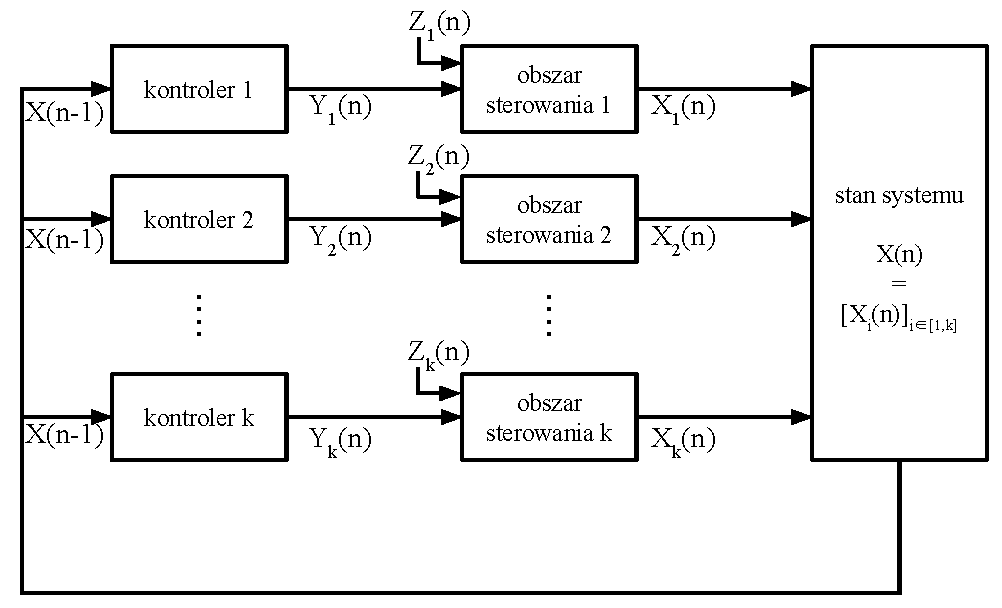
\includegraphics[width=0.8\textwidth]{images/model.pdf}
    \caption{Model systemu sterowania}
    \label{fig:model}
\end{figure}

\begin{equation}
	\begin{array}{c}
		U_i (n) = \left[ u_{i, j} (n) \right]_{j \in <1,s>}\\
		i \in <1,o>\\
		u_{i, j} (n) \in \left\{ \textrm{CZERWONY, CZERWONO-ZOLTY, ZIELONY, ZOLTY} \right\}\\
		o \in \mathbb{N}\\
		s \in \mathbb{N}
	\end{array}
\end{equation}

\begin{math} n \end{math} \textrm{ -- chwila czasu, gdzie czas pomiędzy kolejnymi chwilami czasu to }
\begin{math} t_{n+1} - t_{n} = \delta t = 1s \end{math}

\begin{math} u_{i,j} (n) \end{math} \textrm{ -- stan j-tego sygnalizatora w i-tym obszarze w chwili n}

\begin{math} o \end{math} -- liczba obszarów sterowania

\begin{math} s \end{math} -- liczba sygnalizatorów w obszarze

\begin{equation}
	\begin{array}{c}
		Z_i (n) = \left[ z_{i, j} (n) \right]_{j \in <1,r>}\\
		i \in <1,o>\\
		z_{i, j} (n) \in \mathbb{N}\\
		r \in \mathbb{N}
	\end{array}
\end{equation}

\begin{math} z_{i,j} (n) \end{math} \textrm{ -- przepływ pojazdów z kierunku j w i-tym obszarze w chwili n [pojazdy/godzina]}

\begin{math} r \end{math} -- liczba wlotów do danego obszaru sterowania

\begin{equation}
	\begin{array}{c}
		X_i (n) = \left[
			\begin{array}{c}
				x_{i, j, 1} (n) \\ x_{i, j, 2} (n) \\ x_{i, j, 3} (n)
			\end{array}
		\right]_{j \in <1,s>}\\
		i \in <1,o>\\
		x_{i, j, 1} (n) \in \mathbb{N}\\
		x_{i, j, 2} (n) \in \mathbb{N}\\
		x_{i, j, 3} (n) \in \left\{ \textrm{CZERWONY, CZERWONO-ZOLTY, ZIELONY, ZOLTY} \right\}
	\end{array}
\end{equation}

\begin{math} x_{i, j, 1} (n) \end{math} \textrm{ -- przepływ na dojeździe do j-tego sygnalizatora w i-tym obszarze [pojazdy/godzina]}

\begin{math} x_{i, j, 2} (n) \end{math} \textrm{ -- kolejka przed j-tym sygnalizatorem w i-tym obszarze [liczba pojazdów]}

\begin{math} x_{i, j, 3} (n) \end{math} \textrm{ -- stan j-tego sygnalizatora w i-tym obszarze}

Równanie stanu można zdefiniować jako:
\begin{equation}
	\begin{array}{c}
		x_{i, j, 1} (n+1) = \frac{in_{i, j} (n)}{3600} \\
		x_{i, j, 2} (n+1) = x_{i, j, 2} (n) + x_{i, j, 1} (n) - \frac{out_{i, j} (n)}{3600}\\
		x_{i, j, 3} (n+1) = u_{i, j} (n)
	\end{array}
\end{equation}
gdzie:

\begin{math} in_{i, j} (n) \end{math} \textrm{ -- przepływ pojazdów zbliżających się do j-tego sygnalizatora w i-tym obszarze w chwili n [liczba pojazdów/godzina]}

\begin{math} out_{i, j} (n) \end{math} \textrm{ -- przepływ pojazdów mijających j-ty sygnalizator w i-tym obszarze w chwili n [liczba pojazdów/godzina]}

\vspace{0.5cm}
Wyjście sterowanego obiektu jest odzwierciedleniem stanu obiektu:
\begin{equation}
	\begin{array}{c}
		Y_i (n) = X_i (n)
	\end{array}
\end{equation}


\section{Wymagania sterowania ruchem drogowym}
\label{sec:model_ograniczenia}
Ograniczenia dotyczące sterowania ruchem drogowym zostały ustalone w rozporządzeniu ministra infrastruktury \cite{rozporzadzenie}. Wymagania te można sprowadzić do zestawu wymagań formalnych i wymagań bezpieczeństwa:
\subsection{Wymagania formalne}
\begin{itemize}
	\item Sekwencja sygnałów czerwony, czerwono-żółty\footnote{sygnał czerwony z żółtym, przygotowanie do jazdy}, zielony, żółty, czerwony
	\item Długość sygnału żółtego powinna wynosić 3 sekundy (wzór \ref{formalne:zolty})
	\item Długość sygnału czerwono-żółtego powinna wynosić 1 sekundę (wzór \ref{formalne:czerwono_zolty})
	\item Dla sygnalizacji akomodacyjnej/acyklicznej minimalna długość sygnału zielonego to 5 sekund (wzór \ref{formalne:czerwono_zolty})
\end{itemize}

\begin{equation}
	\label{formalne:zolty}
	x_{i, j, 3} (n) = x_{i, j, 3} (n-1) = x_{i, j, 3} (n-2) = ZOLTY \Longrightarrow \left\{
	\begin{array}{c}
		x_{i, j, 3} (n-3) = ZIELONY\\
		x_{i, j, 3} (n+1) = CZERWONY
	\end{array}
\end{equation}

\begin{equation}
	\label{formalne:czerwono_zolty}
	x_{i, j, 3} (n) = CZERWONO-ZOLTY \Longrightarrow \left\{
	\begin{array}{c}
		x_{i, j, 3} (n-1) = CZERWONY\\
		x_{i, j, 3} (n+1) = ZIELONY\\
		x_{i, j, 3} (n+2) = ZIELONY\\
		x_{i, j, 3} (n+3) = ZIELONY\\
		x_{i, j, 3} (n+4) = ZIELONY\\
		x_{i, j, 3} (n+5) = ZIELONY
	\end{array}
\end{equation}

\subsection{Wymagania bezpieczeństwa}
Rozporządzenie definiuje podział par strumieni ruchu na strumienie niekolizyjne, strumienie kolizyjne o dopuszczalnym jednoczesnym zezwoleniu na ruch oraz strumienie kolizyjne o niedopuszczalnym jednoczesnym zezwoleniu na ruch. Ze względów bezpieczeństwa, na potrzeby opracowywanego systemu przyjęto, że strumienie kolizyjne nigdy nie mogą otrzymać jednoczesnego zezwolenia na ruch.

Zdefiniowano metodę obliczania czasów międzyzielonych dla kolizyjnych par strumieni. Zapewniają one minimalny czas w którym strumień ewakuujący się zdąży minąć punkt kolizji zanim osiągnie go strumień dojeżdżający. Minimalny czas międzyzielony wyznacza się na podstawie czasu trwania sygnału żółtego dla strumienia ewakuującego się, czasu ewakuacji strumienia ewakuującego się oraz czasu dojazdu strumienia dojeżdżającego.

\begin{equation}
	t^{min}_{m} (i,j) = t_{z} + t_{e} (i,j) - t_{d} (i,j)
\end{equation}

\begin{math} t^{min}_{m} (i,j) \end{math} \textrm{ -- minimalny czas międzyzielony dla pary strumieni (i,j) [s]}

\begin{math} t_{z} \end{math} \textrm{ -- długość sygnału żółtego dla strumienia ewakuującego się [s]}

\begin{math} t_{e} (i,j) \end{math} \textrm{ -- czas ewakuacji strumienia i poza punkt kolizji ze strumieniem j [s]}

\begin{math} t_{d} (i,j) \end{math} \textrm{ -- czas dojazdu strumienia j do punktu kolizji ze strumieniem i [s]}

\begin{math} t^{min}_{m} (i,j) = 0 \end{math} \textrm{ jeśli obliczona wartość jest mniejsza od 0}

\begin{equation}
	t_{e} (i,j) = \frac{s_{e} (i,j) + I_p}{v_{e} (i)}
\end{equation}

\begin{math} s_{e} (i,j) \end{math} \textrm{ -- droga strumienia ewakuującego się od linii zatrzymania do punktu kolizji[m]}

\begin{math} I_p \end{math} \textrm{ -- wartość wydłużająca drogę ewakuacji, dla strumienia pojazdów 10 metrów}

\begin{math} v_{e} (i) \end{math} \textrm{ -- prędkość ewakuacji [m/s], prędkość dopuszczalna na wlocie, nie większa niż 14 m/s}

\begin{equation}
	t_{d} (i,j) = \frac{s_{d} (i,j)}{v_{d} (j)} + 1
\end{equation}

\begin{math} s_{d} (i,j) \end{math} \textrm{ -- droga strumienia dojeżdżającego od linii zatrzymania do punktu kolizji [m]}

\begin{math} v_{d} (i) \end{math} \textrm{ -- prędkość ewakuacji [m/s], prędkość dopuszczalna na wlocie}